\chapter{MODEL DEVELOPMENT} \label{label:modeldevelopment}

\graphicspath{{./figures/}}

\section{Physical Setup}
Being a salt water species, macroalgae cultivation occurs primarily in the ocean, with the exception of the initial stage of growth, where microscopic kelp spores are inoculated onto a thread in a small laboratory pool.
This thread is then wrapped around a large rope, which is placed in the ocean and generally suspended by buoys in one of two configurations: horizontal or vertical.
Thus far, I am primarily concerned with modeling the vertical rope case, in which the kelp plants extend radially outward from the rope in all directions, which are made up of a single frond (leaf), stipe (stem) and holdfast (root structure).
We consider a rectangular grid of such vertical ropes. 
Plants extending from each rope will shade both themselves and their neighbors
to varying degrees based on the depth of the kelp, the rope spacing, the angle
of incident light on the surface and the nature of scattering in the water.
In addition, light will be naturally absorbed by the water to varying degrees as determined by the clarity of the water.

\begin{figure}[H]
	\centering
	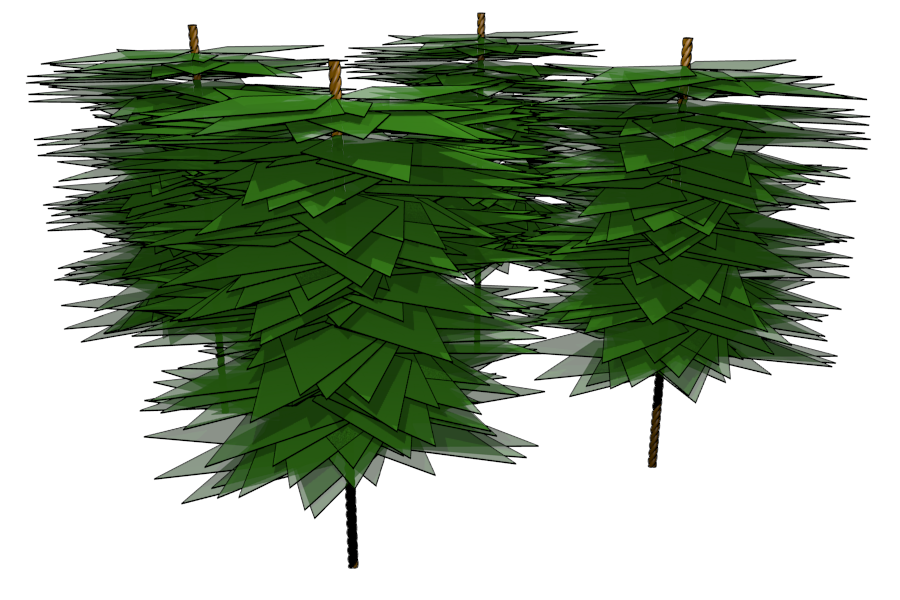
\includegraphics[width=3.5in]{kelp_array}
	\captionof{figure}{$4\times 4$ array of vertical kelp ropes}
\end{figure}
\subsection{Coordinate System}
For all of our three dimensional analysis, we will use the absolute coordinate system defined in figure \ref{fig:3dcoords}.
In the following sections, we will wish to convert between Cartesian and spherical coordinates, which we will do using the following formulas.
\begin{align}
	\begin{split}
		x & = r\sin\phi\cos\theta \\
		y & = r\sin\phi\sin\theta \\
		z & = r\cos\phi \\
	\label{eqn:coords}
	\end{split}
\end{align}

Therefore, for some function $f(x,y,z)$, we can write its derivative along a path in spherical coordinates in terms of Cartesian coordinates using the chain rule.
\begin{equation}
	\frac{\partial f}{\partial r} 
	=\frac{\partial f}{\partial x}\frac{\partial x}{\partial r} 
	+ \frac{\partial f}{\partial y}\frac{\partial y}{\partial r} 
	+ \frac{\partial f}{\partial z}\frac{\partial z}{\partial r}
\end{equation}
Then, calculating derivatives from \eqref{eqn:coords}, we get
\begin{equation}
	\frac{\partial f}{\partial r} 
	=\frac{\partial f}{\partial x}\sin\phi\cos\theta
	+ \frac{\partial f}{\partial y}\sin\phi\sin\theta
	+ \frac{\partial f}{\partial z}\cos\phi
	\label{eqn:partials}
\end{equation}
\begin{figure}[H]
	\centering
	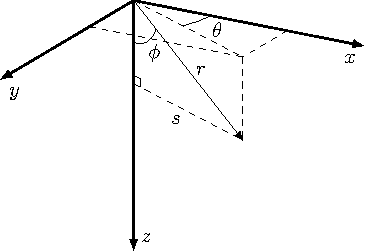
\includegraphics[width=3in]{3d_coords}
	\caption{Downward-facing right-handed coordinate system with radial distance $r$ from the origin, distance $s$ from the $z$ axis, zenith angle $\phi$ and azimuthal angle $\theta$}
	\label{fig:3dcoords}
\end{figure}

\subsection{Domain}

Let the domain be defined as
\begin{equation}
  \begin{split}
    D = \big\{
    \vec{x} \in \RR^3 :\, &\xmin \leq \vec{x} \cdot \hat{x} \leq \xmax \\
    \mbox{ and } &\ymin \leq \vec{x} \cdot \hat{y} \leq \ymax \\
    \mbox{ and } &\zmin \leq \vec{x} \cdot \hat{z} \leq \zmax
    \big\}
  \end{split}
\end{equation}

Let the surface and bottom of the domain be denoted respectively by
\begin{align}
  S &= \left\{\vec{x_s} \in D: \vec{x_s} \cdot \hat{z} = 0 \right\} \\
  B &= \left\{\vec{x_b} \in D: \vec{x_b} \cdot \hat{z} = 0 \right\}
\end{align}

\section{Kelp Model}

\subsection{Frond shape}
\label{sec:shape}

% \begin{figure}[h]
%   \centering
%   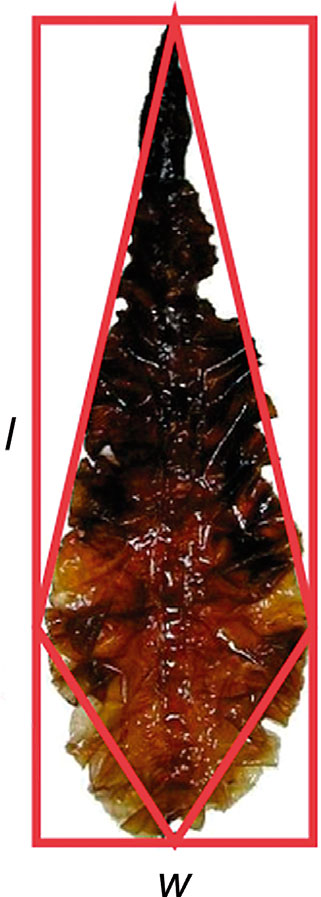
\includegraphics[width=0.7\textwidth]{kelp_photo/kite}
%   \caption{Kite-like shape of \textit{Saccharina Latissima}}
% \end{figure}

\begin{figure}[h]
	\centering
  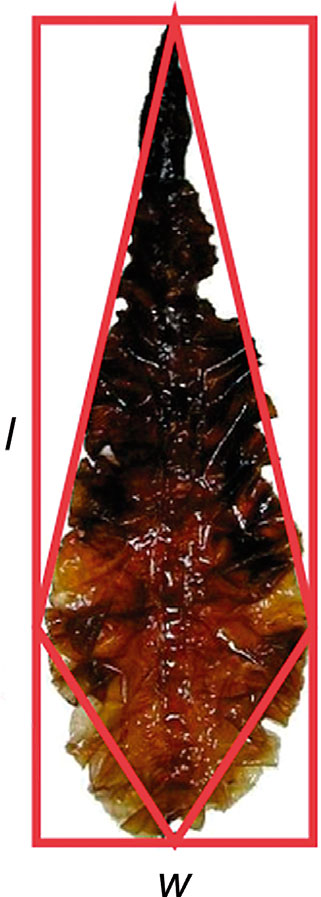
\includegraphics[width=1.2in]{kelp_photo/kite}
  %TODO: Cite this?
  \qquad
	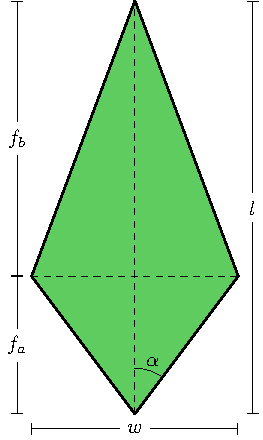
\includegraphics[width=2in]{frond}
	\captionof{figure}{Simplified kite-shaped frond}
	\label{fig:frond}
\end{figure}

We assume the frond is a kite with length $l$ from base to tip, and width $w$ from left to right.
 %In figure \ref{fig:frond}, the base is shown at the bottom and the tip is shown at the top.
 The shortest distance from the base to the diagonal connecting the left and right corners is called $f_a$, and the shortest distance from that diagonal to the tip is called $f_b$.
 We have
 \begin{equation}
	 f_a + f_b = l
 \end{equation}
When considering a whole population with varying sizes, it is more convenient to specify ratios than absolute lengths.
Let the following ratios be defined.
\begin{align}
	f_r &= \frac{l}{w} \\
	f_s &= \frac{f_a}{f_b}
\end{align}
These ratios are assumed to be consistent among the entire population, making all fronds geometrically similar.
With these definitions, the shape of the frond can be fully specified by $l$, $f_r$, and $f_s$.
It is possible, then, to redefine $w$, $f_a$ and $f_b$ as follows from the preceding formulas.

\begin{align}
	w &= \frac{l}{f_r} \\
	f_a &= \frac{lf_s}{1+f_s} \\
	f_b &= \frac{l}{1+f_s}
\end{align}

The angle $\alpha$, half of the angle at the base corner, is also important in our analysis.
Using the above equations,
\begin{equation}
	\alpha = \tan^{-1}\left(\frac{2f_rf_s}{1+f_s}\right)
\end{equation}

The area of the frond is given by
\begin{equation}
  A = \frac{lw}{2} = \frac{l^2}{2f_r}.
\end{equation}

Likewise, if the area is known, then the length is
\begin{equation}
  l = \sqrt{2Af_r}
  \label{eqn:length-from-area}
\end{equation}

\subsection{Length distribution}

% TODO: Normal distribution
We assume that frond lengths are normally distributed.

\subsection{Frond angle distribution}
\label{sec:angle_dist}
We assume the frond angle varies according to the von Mises distribution, which is the periodic analogue of the normal distribution.
It is defined on $[-\pi,\pi]$ rather than $(-\infty,\infty)$.
It has two parameters, $\mu$ and $\kappa$, which shift and sharpen the
distribution respectively.
$\kappa$ can be considered analogous to $1/\sigma$ in the normal distribution.
Here, we use $\mu = \theta_w$ and $\kappa = v_w$.

The PDF for this distribution is
\begin{equation}
	P_{\theta_f}(\theta_f) = \frac{\exp\left(v_w\cos(\theta_f-v_w)\right)}{2\pi I_0(v_w)}
\end{equation}
where $I_0(x)$ is the modified Bessel function of the first kind of order 0.
Notice that unlike the normal distribution, the von Mises distribution approaches a \textit{non-zero} uniform distribution as $\kappa$ approaches 0.
\begin{equation}
	\displaystyle \lim_{v_w \to 0}P_{\theta_f}(\theta_f) = \frac{1}{2\pi} \;\forall\, \theta_f \in [-\pi,\pi]
\end{equation}
The idea behind using this distribution is that with zero current velocity, the frond angles should be distributed uniformly, while as current velocity increases, they should be increasingly likely to be pointing in the direction of the current.
Note that $\theta_w$ and $v_w$ are functions of position.
For a given depth layer, we will use the average water velocity for that depth.

\begin{figure}[h]
	\centering
	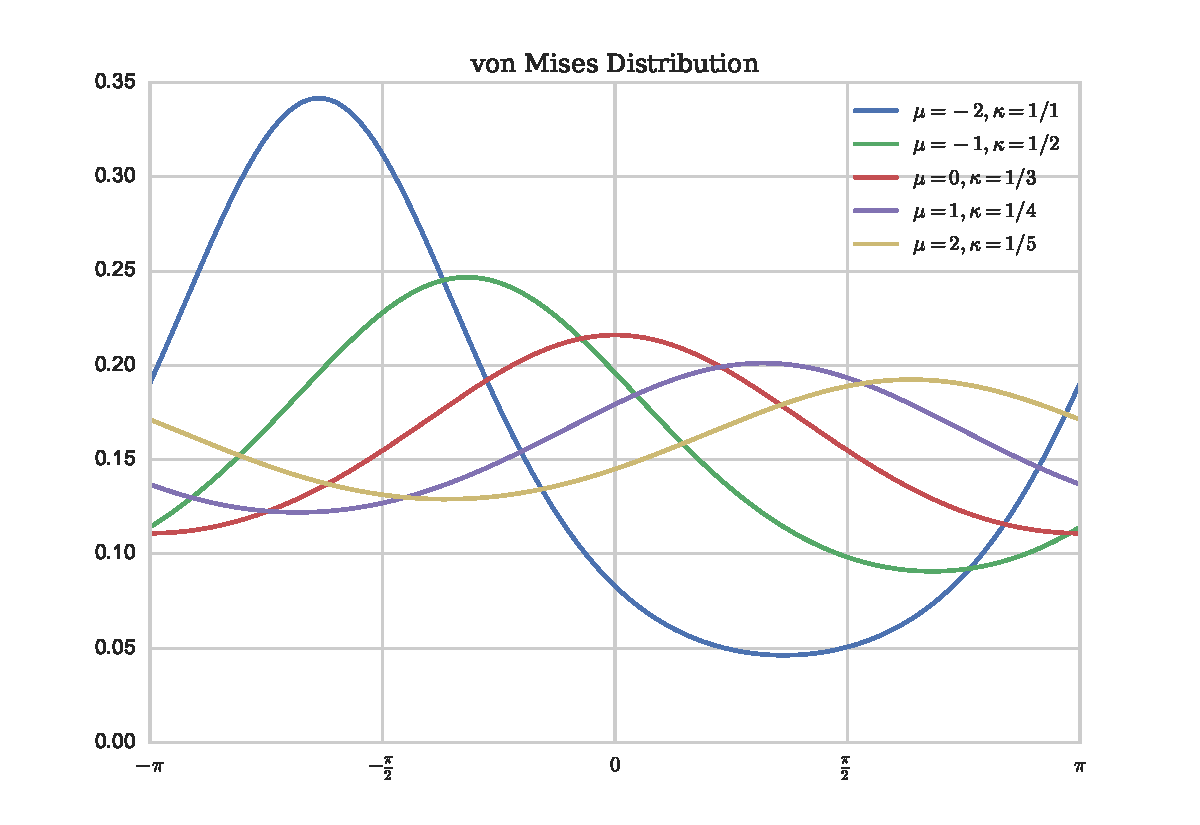
\includegraphics[width=.75\linewidth]{vonmises_2}
	\captionof{figure}{von Mises distribution for a variety of parameters}
	\label{fig:vonmises}
\end{figure}

\subsection{Combined 2D length-angle distribution}
\label{sec:2d_dist}
The previous two distributions can reasonably be assumed to be independent of one another. That is, the angle of the frond does not depend on the length, or vice versa.
Therefore, the probability of a frond simultaneously having a given frond length and angle is the product of their individual probabilities.

Given independent events $A$ and $B$,
\begin{equation}
	\label{eq:ind_prob}
	P(A \cap B) = P(A)P(B)
\end{equation}
Then the probability of frond length $l$ and frond angle $\theta_f$ coinciding is 
\begin{equation}
	P_{2D}(\theta_f,l) = P_{\theta_f}(\theta_f) \cdot L(l)
\end{equation}
A contour plot of this 2D distribution for a specific set of parameters is shown in figure \ref{fig:dist_2d}, where probability is represented by color in the 2D plane.
Darker green represents higher probability, while lighter beige represents lower probability.
In figure \ref{fig:kelp_sample}, 50 samples are drawn from this distribution and plotted.

It is important to note that if $P_{\theta_f}$ were dependent on $l$, the above definition of $P_{2D}$ would no longer be valid.
For example, it might be more realistic to say that larger fronds are less likely to bend towards the direction of the current.
In this case, \eqref{eq:ind_prob} would no longer hold, and it would be necessary to use the following more general relation.
\begin{equation}
	P(A \cap B) = P(A)P(B|A) = P(B)P(B|A)
\end{equation}
This is currently not taken into consideration in this model.

\begin{figure}[h]
	\centering
	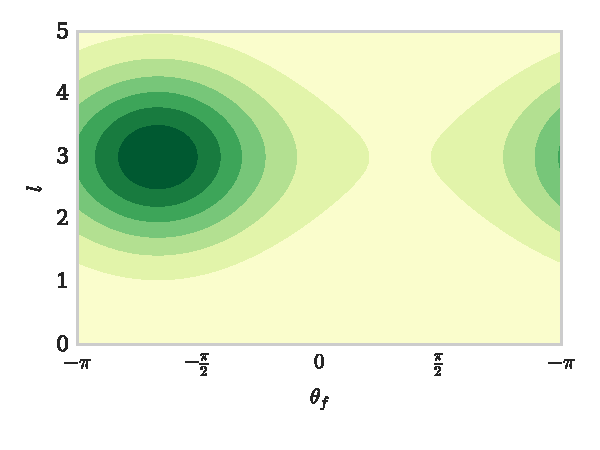
\includegraphics[width=.75\linewidth]{prob_2d}
	\vspace{-3em}
	\captionof{figure}{2D length-angle probability distribution with $\theta_w=2\pi/3,v_w=1$}
	\label{fig:dist_2d}
\end{figure}

\begin{figure}[h]
	\centering
	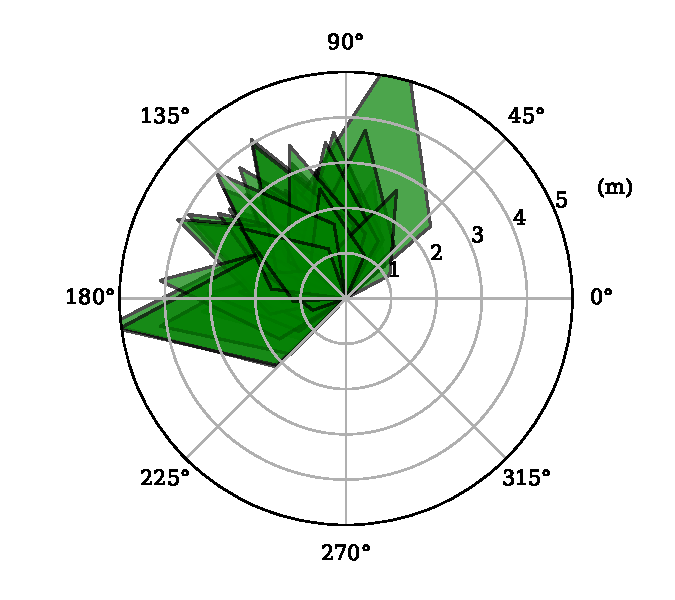
\includegraphics[width=.75\linewidth]{kelp_sample}
	\vspace{-2em}
	\captionof{figure}{A sample of 50 kelp fronds with length and angle picked from the distribution above with $f_s=0.5$ and $f_r=2$.}
	\label{fig:kelp_sample}
\end{figure}


\section{Light Model}

\subsection{Optical Definitions}
One of the most fundamental quantities in optics is radiant flux $\Phi$, which is the has units of energy per time.
The quantity of primary interest in modeling the light field is radiance $L$, which is defined as the radiant flux per steradian per projected surface area perpendicular to the direction of propagation of the beam.
That is,
\begin{equation}
	L = \frac{d^2\Phi}{dA d\omega}
\end{equation}
We must now define a few inherent optical properties (IOPs) which depend only on the medium of propagation.

\subsection{Characteristic Rays}
Consider a fixed position $\vec{x}$ and direction $\vec{\omega}$ such that
$\vec{\omega} \cdot \hat{z} \neq 0$.

% TODO: Just call $\vec{x_0}$ a point, not a function. Call it the projection to the surface.

Let $\vec{l}(\vec{x}, \vec{\omega}, s)$ denote the linear path containing $\vec{x}$
with initial z coordinate given by
\begin{equation}
  z_0 =
   \begin{cases}
    0, & \vec{\omega} \cdot \hat{z} < 0 \\
    \zmax, & \vec{\omega} \cdot \hat{z} > 0
  \end{cases}
\end{equation}

Then,
\begin{equation}
  \vec{l}(\vec{x}, \vec{\omega}, s) = \frac{1}{\tilde{s}} (s\vec{x} + (\tilde{s} - s)\vec{x_0}(\vec{x}, \vec{\omega}))
\end{equation}

where
\begin{equation}
  \vec{x_0}(\vec{x}, \vec{\omega}) = \vec{x} - \tilde{s} \vec{\omega}
\end{equation}
is the origin of the ray, and 

\begin{equation}
  \tilde{s} = \frac{\vec{x} \cdot \hat{z} - z_0}{\vec{\omega} \cdot \hat{z}}
\end{equation}
is the path length from $\vec{x_0}(\vec{x}, \vec{\omega})$ to $\vec{x}$.

\subsection{Colloquial Description}
Denote the radiance at $\vec{x}$ in the direction $\vec{\omega}$ by $L(\vec{x}, \vec{\omega})$.
As light travels along $\vec{l}(\vec{x}, \vec{\omega}, s)$, interaction with the
medium produces three phenomena of interest:
\begin{enumerate}
  \item Radiance is decreased due to absorption.
  \item Radiance is decreased due to scattering out of the path to other
    directions.
  \item Radiance is increased due to scattering into the path from other
      directions.
\end{enumerate}

\subsection{IOPs}
These phenomena are governed by three inherent optical properties (IOPs) of the
medium.
The absorption coefficient $a(\vec{x})$ (units m$^{-1}$) defines the
proportional loss of radiance per unit length.
The scattering coefficient $b$ (units m$^{-1}$), defines the proportional loss
of radiance per unit length, and is assumed to be constant over space.

The volume scattering function (VSF) $\beta(\Delta): [-1, 1] \to \RR^+$ (units sr$^{-1}$) defines the probability of light scattering at any given angle from its source.
Formally, given two directions $\vec{\omega}$ and $\vec{\omega}'$, $\beta(\vec{\omega} \cdot \vec{\omega}')$ is the probability density of light scattering from $\vec{\omega}$ into $\vec{\omega}'$ (or vice-versa).
Of course, since a single direction subtends no solid angle, the probability of scattering occuring exactly from $\vec{\omega}$ to $\vec{\omega}'$ is 0.
Rather, we say that the probability of radiance being scattered from a direction $\omega$ into an element of solid angle $\Omega$ is $\int_\Omega \beta(\vec{\omega} \cdot \vec{\omega}')\, d\vec{\omega}'$.

The VSF is normalized such that
\begin{equation}
  \int_{-1}^1\beta(\Delta)\, d\Delta=\frac{1}{2\pi},
\end{equation}
so that for any $\omega$,
\begin{equation}
  \int_{4\pi}\beta(\vec{\omega}\cdot\vec{\omega}')\, d\vec{\omega}' = 1.
\end{equation}
i.e., the probability of light being scattered to some direction on the unit sphere is 1.

\subsection{Equation of Transfer}
Then, combining these phenomena, the Radiative Transfer equation along
$\vec{l}(\vec{x}, \vec{\omega})$ becomes
\begin{equation}
  \label{eqn:rte1d}
  \frac{dL}{ds}(\vec{l}(\vec{x}, \vec{\omega}, s), \vec{\omega})
  = -(a(\vec{x}) + b)L(\vec{x}, \vec{\omega})
  + b \int_{4\pi} \beta(\vec{\omega}\cdot\vec{\omega}') L(\vec{x})\, d\omega',
\end{equation}
where $\int_{4\pi}$ denotes integration over the unit sphere.

Now, we have
\begin{align*}
  \frac{dL}{ds}(\vec{l}(\vec{x}, \vec{\omega}, s), \vec{\omega})
    &= \frac{d\vec{l}}{ds}(\vec{x}, \vec{\omega}, s) \cdot \nabla L(\vec{x}, \vec{\omega}', \vec{\omega}) \\
    &= \vec{\omega} \cdot \nabla L(\vec{x}, \vec{\omega})
\end{align*}

Then, the general form of the Radiative Transfer Equation is
\begin{equation}
  \vec{\omega} \cdot \nabla L(\vec{x}, \vec{\omega})
  = -(a(\vec{x}) + b)L(\vec{x}, \vec{\omega})
  + b \int_{4\pi} \beta(\vec{\omega}\cdot\vec{\omega}') L(\vec{x}, \vec{\omega}')\, d\omega'
\end{equation}

or, equivalently,
\begin{equation}
  \vec{\omega} \cdot \nabla L(\vec{x}, \vec{\omega})
  + a(\vec{x})L(\vec{x}, \vec{\omega})
  = b \left(
    \int_{4\pi} \beta(\vec{\omega}\cdot\vec{\omega}') L(\vec{x}, \vec{\omega}')\, d\omega'
    - L(\vec{x}, \vec{\omega})
  \right)
\end{equation}

\subsection{Boundary Conditions}

We use periodic boundary conditions in the $x$ and $y$ directions.
\begin{align}
  L\left((\xmin, y, z), \vec{\omega}\right) &= L\left((\xmax, y, z), \vec{\omega}\right) \\
  L\left((x, \ymin, z), \vec{\omega}\right) &= L\left((x, \ymax, z), \vec{\omega}\right)
\end{align}

In the $z$ direction, we specify a spatially uniform downwelling light just
under the surface of the water by a function $f(\vec{\omega})$.
Or if $\zmin>0$, then the radiance at $z=\zmin$ should be specified instead (as opposed to the radiance at the first grid cell center).

Further, we assume that no upwelling light enters the domain from the bottom.
\begin{align}
  L(\vec{x_s}, \vec{\omega}) &= f(\omega) \mbox{ if } \vec{\omega} \cdot \hat{z} > 0\\ 
  L(\vec{x_b}, \vec{\omega}) &= 0 \mbox { if } \vec{\omega} \cdot \hat{z} < 0
\end{align}
 
\section{Total Light Absorption}
Once the radiance $L$ is calculated everywhere, the irradiance is
\begin{equation}
  I(\vec{x}) = \int_{4\pi}L(\vec{x},\vec{\omega})\, d\omega.
\end{equation}

Then, the light absorbed by the fronds is calculated by multiplying the kelp distribution by the irradiance.
(This needs to be explained more, and needs to come after the super-individual section).
%TODO: Do this right.
